\documentclass{article}
\usepackage{tikz}
\usepackage{amsmath}
\usepackage{graphicx}
\usepackage[colorlinks=true, citecolor=blue, linkcolor=blue, urlcolor=blue]{hyperref}
\usetikzlibrary{decorations.pathmorphing, arrows.meta, positioning, calc, fit, backgrounds}

\begin{document}

\title{Analysis of a Doubly Spread Channel}
\author{}
\date{\today}

\maketitle

\section{Theoretical Framework}
This section establishes the physical foundations of acoustic signal distortion. 
A \textbf{Doubly Spread Channel} \cite{stojanovic1996recent, preisig2007acoustic} is driven by two coupled mechanisms: \textbf{Source Kinematics (Heave)} and \textbf{Dynamic Boundary Interaction (Micro-Multipath)}.

\section{Source on the surface}
A surface vessel represents the worst-case scenario for acoustic smearing due to physical coupling with the dynamic boundary.

\subsection{Schematic Diagram}
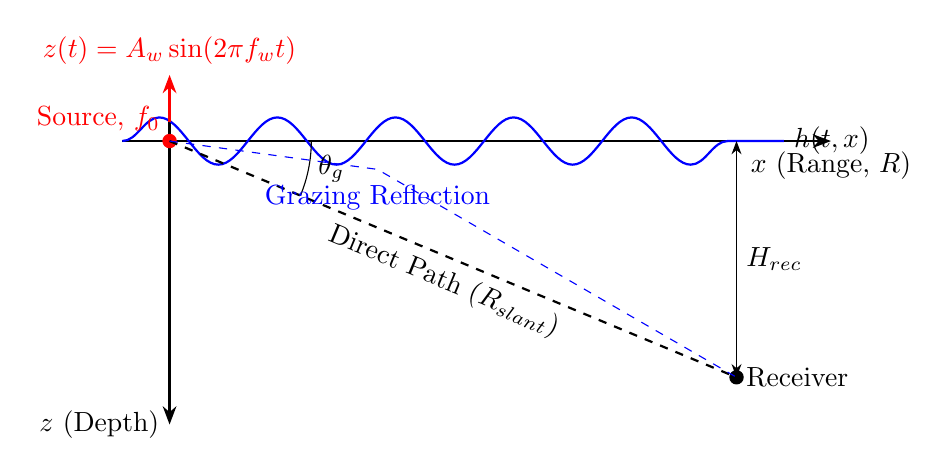
\begin{tikzpicture}[scale=1.2, >=Stealth]

    % Define variables/coordinates
    \def\Range{6}
    \def\Hrec{-2.5}
    
    % Draw axes
    \draw[->, thick] (0, 0.5) -- (0, \Hrec - 0.5) node[left] {$z$ (Depth)};
    \draw[->, thick] (-0.5, 0) -- (\Range + 1, 0) node[below] {$x$ (Range, $R$)};
    
    % Draw rough ocean surface
    \draw[blue, thick, decoration={snake, amplitude=3mm, segment length=15mm}, decorate] 
        (-0.5, 0) -- (\Range + 0.5, 0) node[right, text=black] {$h(t, x)$};
        
    % Source Vessel
    \filldraw[red] (0,0) circle (2pt) node[above left] {Source, $f_0$};
    \draw[->, red, thick] (0, 0.2) -- (0, 0.7) node[above] {$z(t) = A_w \sin(2\pi f_w t)$};
    
    % Receiver
    \filldraw[black] (\Range, \Hrec) circle (2pt) node[right] {Receiver};
    
    % Direct path and angle
    \draw[dashed, thick] (0,0) -- (\Range, \Hrec) node[midway, sloped, below] {Direct Path ($R_{slant}$)};
    \draw (1.5, 0) arc (0:{-atan(2.5/6)}:1.5) node[midway, right] {$\theta_g$};
    
    % Surface interaction path (Shadowing example)
    \draw[blue, dashed] (0,0) -- (2.2, -0.3) -- (\Range, \Hrec);
    \node[blue, align=center] at (2.2, -0.6) {Grazing Reflection};
    
    % Annotate Depth and Range
    \draw[<->] (\Range, 0) -- (\Range, \Hrec) node[midway, right] {$H_{rec}$};
    
\end{tikzpicture}

\subsection{Physical \& Mathematical Breakdown}

\subsubsection{The Grazing Angle}
This subsection calculates the reflection geometry to prove the direct and surface paths overlap.
\begin{equation}
\theta_g = \arctan \left( \frac{H_{rec} - H_{src}}{R} \right)
\end{equation}
For a surface source ($H_{src} \approx 0$) and long range ($R \gg H_{rec}$), $\theta_g \approx 0^\circ$.

\subsubsection{The Transmitted Signal: Source Kinematics}
This models how vertical vessel heave modulates the emitted acoustic wave.
The source emits a pressure wave $p(t)$:
\begin{align}
p(t) &= P_0 \cos(2\pi f_0 t)
\intertext{The heave motion induces a phase shift:}
z(t) &= A_w \sin(2\pi f_w t)
\intertext{Creating a Phase/Frequency Modulated (FM) signal:}
p_{tx}(t) &= P_0 \cos\left(2\pi f_0 t + \beta \sin(2\pi f_w t)\right)
\intertext{Where modulation index $\beta$ is:}
\beta &= \frac{2\pi f_0}{c} A_w \cos\theta_g
\intertext{The resulting time-varying instantaneous frequency $f_i(t)$ is:}
f_i(t) &= \frac{1}{2\pi} \frac{d\Phi}{dt} = f_0 + \Delta f \cos(2\pi f_w t) \\
\Delta f &= \beta f_w = \frac{2\pi f_0 f_w}{c} A_w \cos\theta_g
\end{align}

\subsubsection*{Spectral Expansion (The Bessel Comb)}
This proves the vessel's heave expands the tonal into an infinite series of frequency sidebands \cite{carlson2001}.
Using the Jacobi-Anger expansion:
\[ p_{tx}(t) = P_0 \text{Re} \left\{ \sum_{n=-\infty}^{\infty} J_n(\beta) e^{i 2\pi (f_0 + n f_w) t} \right\} \]
\begin{equation}
p_{tx}(t) = P_0 \sum_{n=-\infty}^{\infty} J_n(\beta) \cos\left( 2\pi (f_0 + n f_w) t \right)
\end{equation}

\subsubsection{Channel Interaction with Dynamic Boundary \& Multipath}
This models how moving waves act as a dynamic scatterer (Doppler) that changes the reflected path.
Because $\theta_g \approx 0^\circ$, the time delay between paths approaches zero ($\Delta \tau \approx 0$).
\begin{align}
p_{rx}(t) &= \frac{1}{R_{dir}} p_{tx}(t - \tau_{dir}) + \frac{V(t)}{R_{surf}} p_{tx}(t - \tau_{surf})
\intertext{Where the time-varying scattering coefficient $V(t)$ is:}
V(t) &= -R_0 \exp\left( i \frac{4\pi f_0}{c} h_s(t) \sin\theta_g \right)
\end{align}
This standard Kirchhoff approximation \cite{bass1979wave, roderick1979doppler} encapsulates the $180^\circ$ phase inversion at the boundary ($-1$), the amplitude loss from roughness ($R_0$), and the Doppler phase shift caused by the changing path length over the moving waves ($\exp$).

\subsubsection{The Smeared Received Signal}
Combining source modulation and channel interaction yields the final smeared equation.
Because $\tau_{dir} \approx \tau_{surf}$, we factor the received field:
\[ p_{rx}(t) \propto p_{tx}(t - \tau_{dir}) \left[ 1 - R_0 \exp\left( i \frac{4\pi f_0}{c} h_s(t) \sin\theta_g \right) \right] \]
\textbf{Conclusions:}
\begin{enumerate}
    \item \textbf{Modulated Carrier:} $p_{tx}$ is FM due to heave.
    \item \textbf{Multiplicative Fading:} The bracketed term causes random amplitude oscillation.
    \item \textbf{Secondary Phase Modulation:} The exponential causes Doppler spread.
\end{enumerate}

\subsubsection{Connection to the Doubly Spread Channel}
This formally defines the environment as a doubly spread acoustic channel:
\begin{enumerate}
    \item \textbf{Delay Spread:} Paths arrive simultaneously, fading multiplicatively.
    \item \textbf{Doppler Spread:} Surface velocity and vessel heave spread frequency.
\end{enumerate}

\section{Source Underwater}
This isolates the source to demonstrate how physical decoupling stabilizes the signal.

\subsection{Schematic}
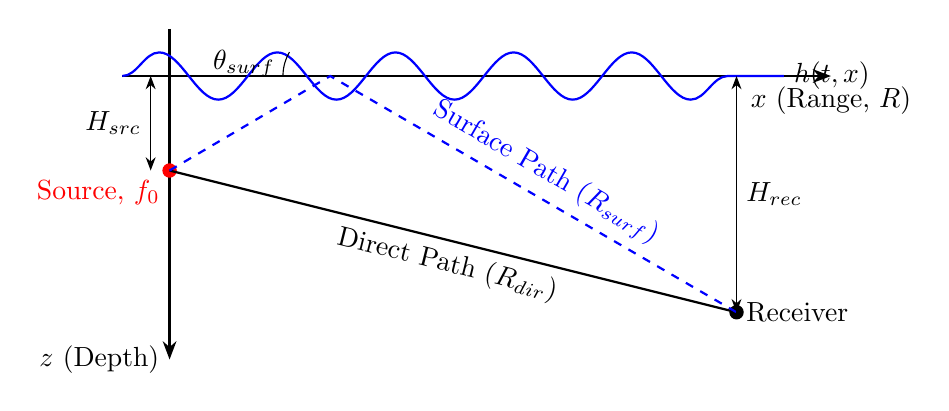
\begin{tikzpicture}[scale=1.2, >=Stealth]

    % Define variables/coordinates
    \def\Range{6}
    \def\Hrec{-2.5}
    \def\Hsrc{-1.0}
    
    % Draw axes
    \draw[->, thick] (0, 0.5) -- (0, \Hrec - 0.5) node[left] {$z$ (Depth)};
    \draw[->, thick] (-0.5, 0) -- (\Range + 1, 0) node[below] {$x$ (Range, $R$)};
    
    % Draw rough ocean surface
    \draw[blue, thick, decoration={snake, amplitude=3mm, segment length=15mm}, decorate] 
        (-0.5, 0) -- (\Range + 0.5, 0) node[right, text=black] {$h(t, x)$};
        
    % Underwater Source Vessel
    \filldraw[red] (0,\Hsrc) circle (2pt) node[below left] {Source, $f_0$};
    \draw[<->] (-0.2, 0) -- (-0.2, \Hsrc) node[midway, left] {$H_{src}$};
    
    % Receiver
    \filldraw[black] (\Range, \Hrec) circle (2pt) node[right] {Receiver};
    
    % Direct path
    \draw[solid, thick] (0,\Hsrc) -- (\Range, \Hrec) node[midway, below, sloped] {Direct Path ($R_{dir}$)};
    
    % Surface interaction path (Resolved Multipath)
    \draw[blue, dashed, thick] (0,\Hsrc) -- (1.7, 0) -- (\Range, \Hrec) node[midway, above, sloped, text=blue] {Surface Path ($R_{surf}$)};
    
    % Grazing Angle at surface
    \draw (1.2, 0) arc (180:{180+atan(\Hsrc/1.7)}:0.5) node[midway, left] {$\theta_{surf}$};
    
    % Annotate Depth and Range
    \draw[<->] (\Range, 0) -- (\Range, \Hrec) node[midway, right] {$H_{rec}$};
    
\end{tikzpicture}

\subsection{Physical \& Mathematical Breakdown}

\subsubsection{Elimination of Source Kinematics}
Operating below the wave base eliminates physical heave ($A_w \approx 0$).
\begin{equation}
\beta = \frac{2\pi f_0}{c} A_w \cos\theta_g \approx 0
\end{equation}
The transmitted signal reverts to a pure tone:
\begin{equation}
p_{tx}(t) = P_0 \cos(2\pi f_0 t)
\end{equation}

\subsubsection{Resolution of Macro-Multipath}
Depth creates significant geometric path differences ($R_{surf} \gg R_{dir}$), creating macroscopic time delays ($\Delta \tau \gg 0$) that break multiplicative interference.

\subsubsection{The Decoupled Received Signal}
The final equation for an underwater source:
\begin{equation}
p_{rx}(t) = \underbrace{ \frac{P_0}{R_{dir}} \cos(2\pi f_0 (t - \tau_{dir})) }_{\text{Direct Path}} + \underbrace{ \frac{P_0 V(t)}{R_{surf}} \cos(2\pi f_0 (t - \tau_{surf})) }_{\text{Surface Echo}}
\end{equation}
The direct path is unmodified, and the surface echo arrives much later, adding additive clutter rather than multiplicative fading.

\clearpage
\section{Flow Diagram}
This outlines the signal processing architecture designed to mitigate smearing.

\resizebox{!}{0.85\textheight}{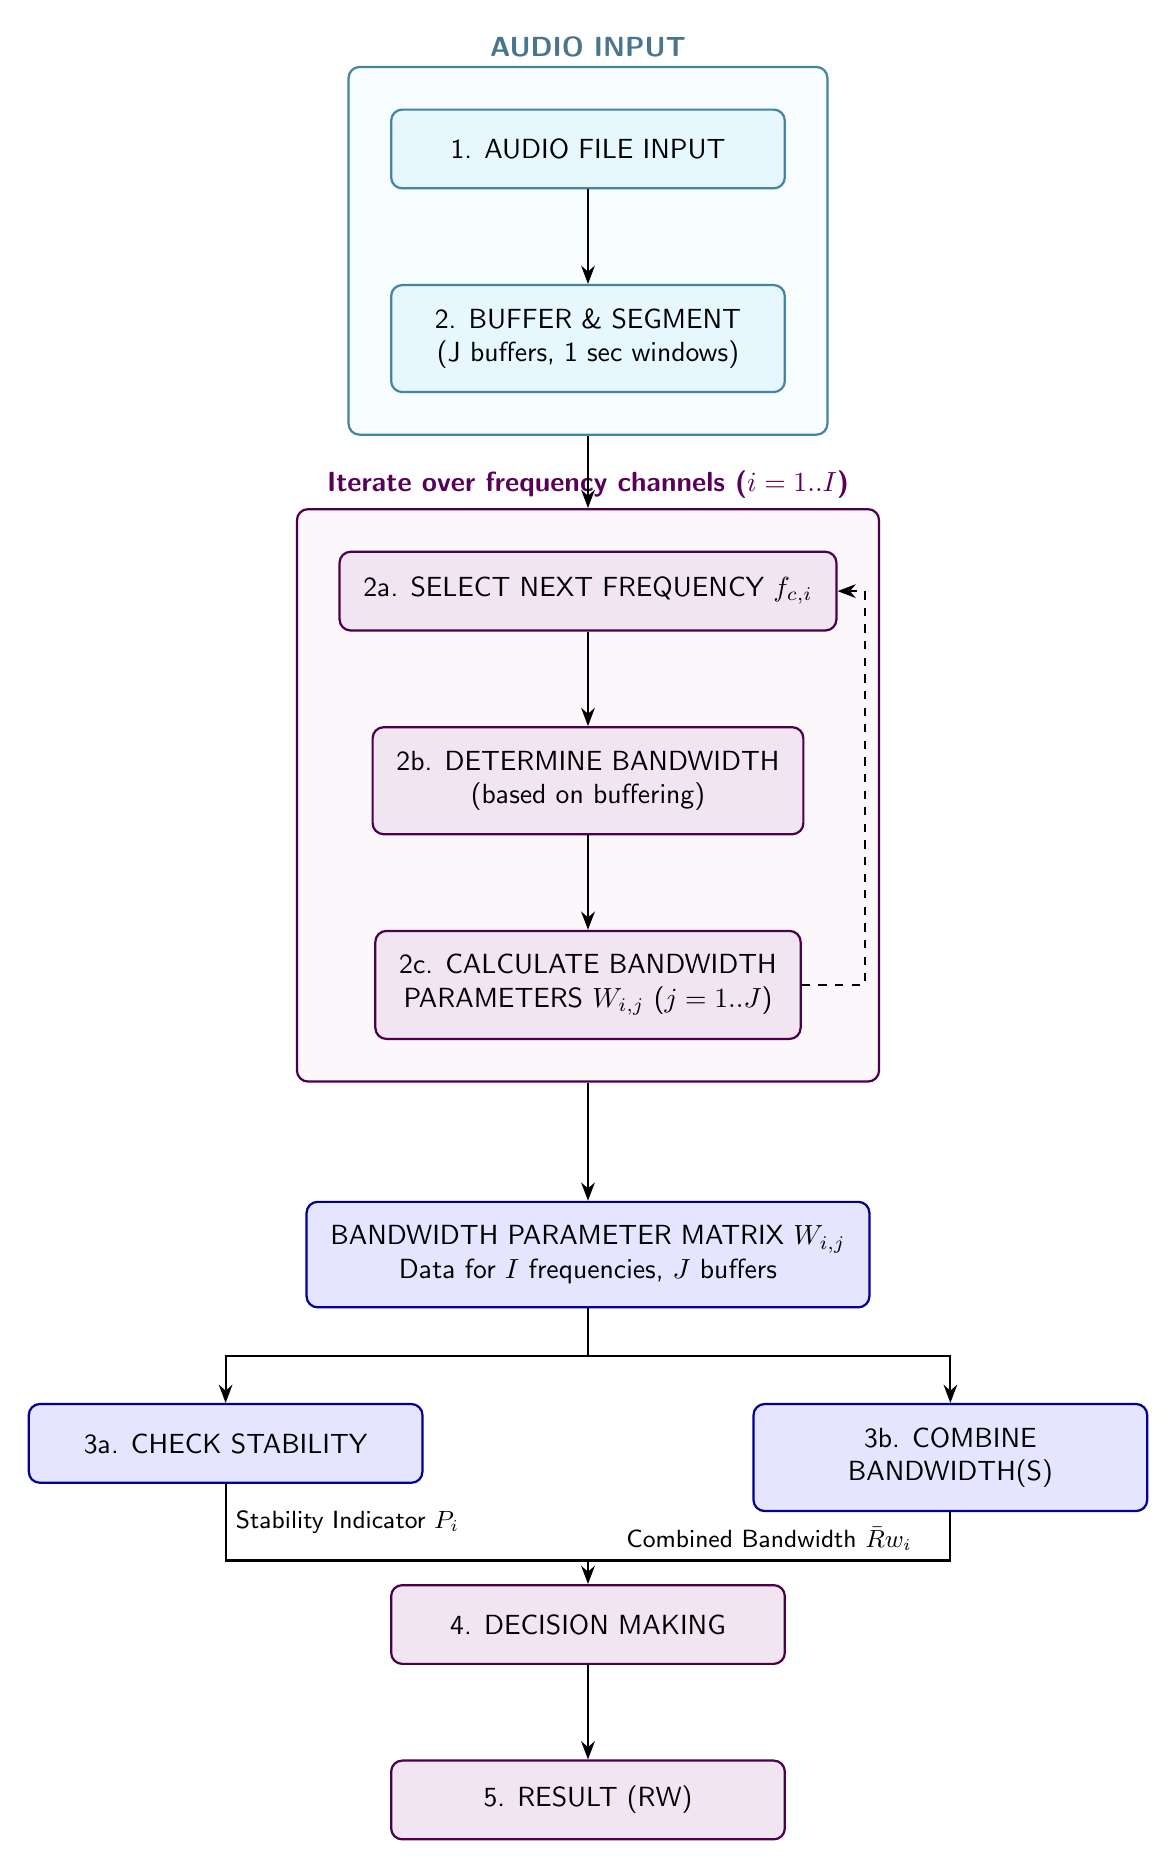
\begin{tikzpicture}[
    >=Stealth,
    node distance=1.2cm and 1.5cm,
    font=\sffamily,
    % Define styles for the different node types
    cyanbox/.style={rectangle, rounded corners, draw=cyan!60!black, fill=cyan!10, thick, text centered, align=center, minimum width=5cm, minimum height=1cm, inner sep=2ex},
    bluebox/.style={rectangle, rounded corners, draw=blue!60!black, fill=blue!10, thick, text centered, align=center, minimum width=5cm, minimum height=1cm, inner sep=2ex},
    purplebox/.style={rectangle, rounded corners, draw=violet!60!black, fill=violet!10, thick, text centered, align=center, minimum width=5cm, minimum height=1cm, inner sep=2ex},
    greenbox/.style={rectangle, rounded corners, draw=green!50!black, fill=green!10, thick, text centered, align=center, minimum height=0.8cm, inner sep=1.5ex},
    cyancontainer/.style={rectangle, rounded corners, draw=cyan!60!black, fill=cyan!3, thick, inner sep=15pt},
    purplecontainer/.style={rectangle, rounded corners, draw=violet!60!black, fill=violet!3, thick, inner sep=15pt},
]

% -------------------------
% Main Flow Nodes
% -------------------------
\node (audio) [cyanbox] {1. AUDIO FILE INPUT};
\node (buffer) [cyanbox, below=of audio] {2. BUFFER \& SEGMENT\\(J buffers, 1 sec windows)};

% Loop Inner Nodes
\node (c1) [purplebox, below=2cm of buffer] {2a. SELECT NEXT FREQUENCY $f_{c,i}$};
\node (c2) [purplebox, below=of c1] {2b. DETERMINE BANDWIDTH\\(based on buffering)};
\node (c3) [purplebox, below=of c2] {2c. CALCULATE BANDWIDTH\\PARAMETERS $W_{i,j}$ ($j=1..J$)};

% Loop Container Box
\begin{scope}[on background layer]
    \node (loopgroup) [purplecontainer, fit=(c1) (c2) (c3), label={[font=\sffamily\bfseries, text=violet!70!black]above:Iterate over frequency channels ($i=1..I$)}] {};
\end{scope}

\node (matrix) [bluebox, below=1.5cm of loopgroup] {BANDWIDTH PARAMETER MATRIX $W_{i,j}$\\Data for $I$ frequencies, $J$ buffers};

% Split Output Nodes
\node (stability) [bluebox, below left=1.2cm and -1.5cm of matrix] {3a. CHECK STABILITY};
\node (combine) [bluebox, below right=1.2cm and -1.5cm of matrix] {3b. COMBINE\\BANDWIDTH(S)};

% Final Nodes
\node (decision) [purplebox, below=3.5cm of matrix] {4. DECISION MAKING};
\node (result) [purplebox, below=of decision] {5. RESULT (RW)};


% Audio Input Container Box
\begin{scope}[on background layer]
    \node (inputgroup) [cyancontainer, fit=(audio) (buffer), label={[font=\sffamily\bfseries, text=cyan!50!black]above:AUDIO INPUT}] {};
\end{scope}


% -------------------------
% Arrow Connections
% -------------------------

% Input group to loop group
\draw[->, thick] (inputgroup.south) -- (loopgroup.north);

% Main flow top
\draw[->, thick] (audio) -- (buffer);

% Loop internals
\draw[->, thick] (c1) -- (c2);
\draw[->, thick] (c2) -- (c3);
% Feedback loop (dashed)
\draw[->, thick, dashed] (c3.east) -- ++(0.8,0) |- (c1.east);

% Loop to matrix
\draw[->, thick] (loopgroup.south) -- (matrix.north);

% Matrix to Split
\coordinate (matrix_split) at ($(matrix.south) + (0,-0.6)$);
\draw[thick] (matrix.south) -- (matrix_split);
\draw[->, thick] (matrix_split) -| (stability.north);
\draw[->, thick] (matrix_split) -| (combine.north);

% Split to Decision
\coordinate (decision_merge) at ($(decision.north) + (0,0.3)$);
\draw[thick] (stability.south) |- (decision_merge) node[near start, right, font=\sffamily\small] {Stability Indicator $P_i$};
\draw[thick] (combine.south) |- (decision_merge) node[near end, above, font=\sffamily\small] {Combined Bandwidth $\bar{R}{w_i}$};
\draw[->, thick] (decision_merge) -- (decision.north);

% Decision to Result
\draw[->, thick] (decision) -- (result);

\end{tikzpicture}}

\begin{thebibliography}{9}
\bibitem{stojanovic1996recent}
M.~Stojanovic, ``Recent advances in high-speed underwater acoustic communications,'' \emph{IEEE Journal of Oceanic Engineering}, vol.~21, no.~2, pp. 125--136, 1996.

\bibitem{preisig2007acoustic}
J.~C. Preisig, ``Acoustic propagation considerations for underwater acoustic communications,'' \emph{IEEE Communications Magazine}, vol.~45, no.~12, pp. 110--117, 2007.

\bibitem{carlson2001}
A.~B. Carlson, P.~B. Crilly, and J.~C. Rutledge, \emph{Communication Systems: An Introduction to Signals and Noise in Electrical Communication}, 4th~ed.\hskip 1em plus 0.5em minus 0.4em\relax McGraw-Hill, 2001.

\bibitem{bass1979wave}
F.~G. Bass and I.~M. Fuks, \emph{Wave Scattering from Statistically Rough Surfaces}.\hskip 1em plus 0.5em minus 0.4em\relax Pergamon Press, Oxford, 1979.

\bibitem{roderick1979doppler}
W.~I. Roderick, ``Doppler spectra of acoustic signals reflected from a moving rough sea surface,'' Ph.D. dissertation, Yale University, New Haven, CT, 1979.
\end{thebibliography}

\end{document}
